\section{Шероховатость}

Шероховатость поверхности --- совокупность неровностей поверхности с относительно мальми шагами, выделенную с помощью базовой длины. Появляется в процессе формообразования.

$R_a$ --- среднее арифметическое отклонение профиля.

\[ R_a = \dfrac{1}{l} \int\limits_0^l |y(x)| \; dx \]

$R_z$ --- высота неровностей профиля по 10 точкам. 5 --- наибольшие выступы, 5 --- наибольшие впадины.

\[ R_z = \dfrac{\sum\limits_{i=1}^5 |y_{pi}| - \sum\limits_{i=1}^5 |y_{vi}|}{5} \]

$R_{\max}$ --- наибольшая высота неровностей профиля. Расстояние между линией выступов профиля и линией впадин профиля.

$S_m$ --- средний шаг неровностей профиля --- среднее значение неровностей профиля в пределах базовой длины.

\begin{figure}
	\centering
	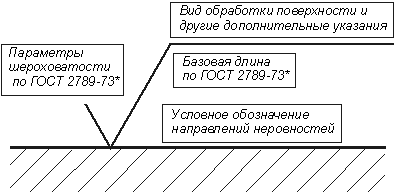
\includegraphics[width=0.7\linewidth]{pic/1_5}
	\caption{Обозначение шероховатости}
	\label{fig:15}
\end{figure}


$S$ --- Средний шаг выступов профиля --- среднее значение выступов профиля в пределах базовой длины.

$t_p$ --- Относительная опорная длина профиля --- отношение опорной длины профиля к базовой длине.

\[ t_p = \dfrac{1}{l} \sum\limits_{i=1}^n b_i \]

\begin{figure}
	\centering
	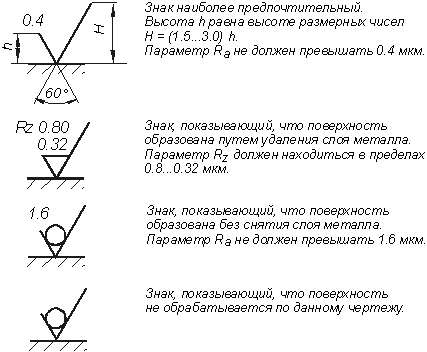
\includegraphics[width=0.7\linewidth]{pic/1_6}
	\caption{Обозначение шероховатости на чертеже.}
	\label{fig:16}
\end{figure}


\section{Резьбовые соединения.}

Приведенный средний диаметр резьбы --- средний диаметр воображаемой идеальной резьбы, которая имеет те же шаг и угол наклона боковых сторон, что и основной или номинальный профиль резьбы, и длину, равную заданной длине свинчивания, которая плотно (без взаимного смещения или натяга) соприкасается с реальной резьбой по боковым сторонам резьбы. Необходим для упрощения допусков контроля резьбы.

\[ d_{2 пр} = d_{2 изм} + f_p + f_{\alpha} \]

\[  D_{2 пр} = D_{2 изм} - (f_p + f_{\alpha})  \]

$f_p$ --- диаметральная компенсация погрешности шага.

Средний диаметр, шаг и угол профиля являются основными параметрами резьбы, т.к. они определяют характер контакта резьбового соединения. Однако вследствие взаимосвязи между отклонениями шага, угла профиля и собственно среднего диаметра допустимые отклонения этих параметров раздельно не нормируют. Устанавливают только суммарный допуск на средний диаметр болта $Td_2$ и гайки $TD_2$, который включает допустимое отклонение собственно среднего диаметра $\bigtriangleup d_2$ и диаметральные компенсации погрешности шага и угла профиля, т.е.

\[ TD_2 = \bigtriangleup D_2 + f_p + f_{\alpha} \]

Условия годности резьбы:

\[ d_{2 изм} \geqslant d_{2 \min}; d_{2 пр} \leqslant d_{2 \max} \]

Пример обозначения резьбы: М12-6g(наружняя); M12-6H(внутренняя)

\section{Зубчатые передачи}

Классификация зубчатых передач:

\begin{enumerate}
	\item Отсчётные --- зубчатые передачи различных счётных механизмов. Основное требование --- высокая кинематическая точность.
	\item Скоростные --- требуется плавность работы.
	\item Силовые --- зубчатые передачи в прокатных станах. Требуется полнота контакта сопряжённых зубьев
\end{enumerate}

Установлено 12 степеней точности.

Нормы точности:

\begin{enumerate}
	\item Кинематическая --- устанавливает разность между действительными и номинальными углами поворота колеса
	\item Плавность работы --- ограничивает погрешность угла поворота колеса при повороте на 1 зуб.
	\item Контактная точность --- Ограничивают неполноту контакта сопряжённых зубьев
\end{enumerate}

Погрешность передаточного отношения:

\[ F_{ior} = (\varphi_{2 действ} - \varphi_{2 ном}) \cdot r [мкм] \]

\begin{figure}
	\centering
	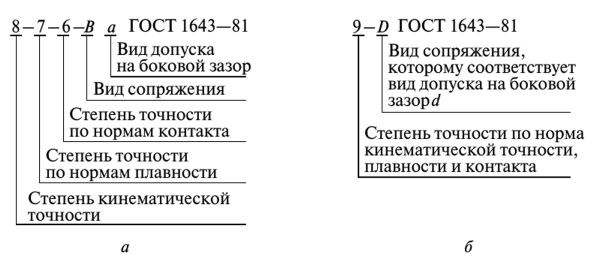
\includegraphics[width=0.7\linewidth]{pic/408}
	\caption{Обозначение точности зубчатого колеса}
	\label{fig:408}
\end{figure}

Принцип комбинирования норм точности --- для одного колеса можно назначать разные точности на разные параметры. Упрощает производство, т. к. последняя операция может улучшать только 1 показатель.

Виды сопряжений зубьев зубчатых колес в передачах

Характер сопряжений зубьев определяется боковым зазором между их нерабочими боковыми поверхностями.

Боковой зазор в передаче отсчитывают по общей нормали к боковым поверхностям зубьев (по линии зацепления). Он необходим для компенсации погрешностей изготовления и сборки передач, для создания расчетных условий смазывания, а также для устранения опасности заклинивания зубьев одного зубчатого колеса во впадинах другого в результате тепловых и силовых деформаций.

